\chapter{ПРОВЕРКА ВЫЧИСЛИТЕЛЬНОЙ ПРОГРАММЫ} \label{ch4}

\section{Интегрирование уравнения движения}

Для численного решения уравнений движения с помощью метода Рунге-Кутты используется код написанный на языке \texttt{c++}.
Перед моделированием достаточно сложных процессов необходимо выяснить насколько точно и правильно считает программа. Для этого было проведено сравнение численных результатов с аналитическими решениями при движении электрона в электрическом поле, а также в скрещенных электромагнитных полях. Также были проведено сравнение расчёта электронного релятивистского потока с независимыми результатами других исследователей.

Было выяснено, что программа написана правильно, т.~к. наблюдалось хорошая сходимость результатов. Более того, были выяснены параметры временной дискретизации. Подробные выкладки и результаты сравнения представлены в приложении \ref{AppendixC}. 



\section{Инициализация плазмы}

\subsection{Задание начальных положений}
\label{sec:MT19937}

Для того чтобы правильно инициализировать систему необходимо выработать алгоритм случайного задания \textit{положений} и \textit{скоростей}. 

Задача задания случайного положения решается путём выбора наиболее хорошего генератора псевдослучайных чисел. Был выбран генератор вихрь Мерсенна с его алгоритмической реализацией MT19937. Причины выбора следующие: данный алгоритм обеспечивает быструю и очень качественную реализацию генерации псевдослучайных чисел. Его период составляет $2^{19937}-1$, а также алгоритм показывает высокие результаты в тесте DIEHARD \cite{matsumoto1998mersenne,sriram2006area}.

Стоить заметить, что использование стандартной функции \texttt{RAND()} в \texttt{c++} неприменимо, т.~к. тогда наблюдаются определенные неслучайные пространственные структуры, что недопустимо \cite{habr_rand}.

\subsection{Задание начальных скоростей согласно распределению Максвелла}
\label{sec:HowToMaxwell}

Для частиц в плазме справедливо распределение Максвелла (за некоторыми частными исключениями). Встаёт задача о задании процедуры случайного задания скорости по заданной функции плотности распределения:
\begin{equation}
f(v) = 4 \pi v^2 \left( \frac{m}{2 \pi T} \right)^{3/2} \exp \left[ - \frac{m v^2/2}{T} \right].
\label{eq:maxwell_dist}
\end{equation}

Алгоритм решения поставленной задачи следующий:
\begin{enumerate}
\item Зная конкретный вид $f(v)$, численно табулируется функция распределения
\begin{equation}
F_i (v_i) = \int\limits_{- \infty}^{v_i} f(v') dv'.
\end{equation}
\item По данным таблицы значений $\left\{ F_i ; v_i  \right\}$, интерполируется функция  $F^{-1}(v) = v(F)$.
\item В силу свойств функции распределения $F \in \left[0,1\right]$. Тогда, очевидно, необходимо задать случайную величину в диапазоне от 0 до 1, подставить в полученную функцию и получить желаемый результат (рисунок \ref{fig:He(T=273)}).
\end{enumerate}

\begin{figure}[h!]
\centering
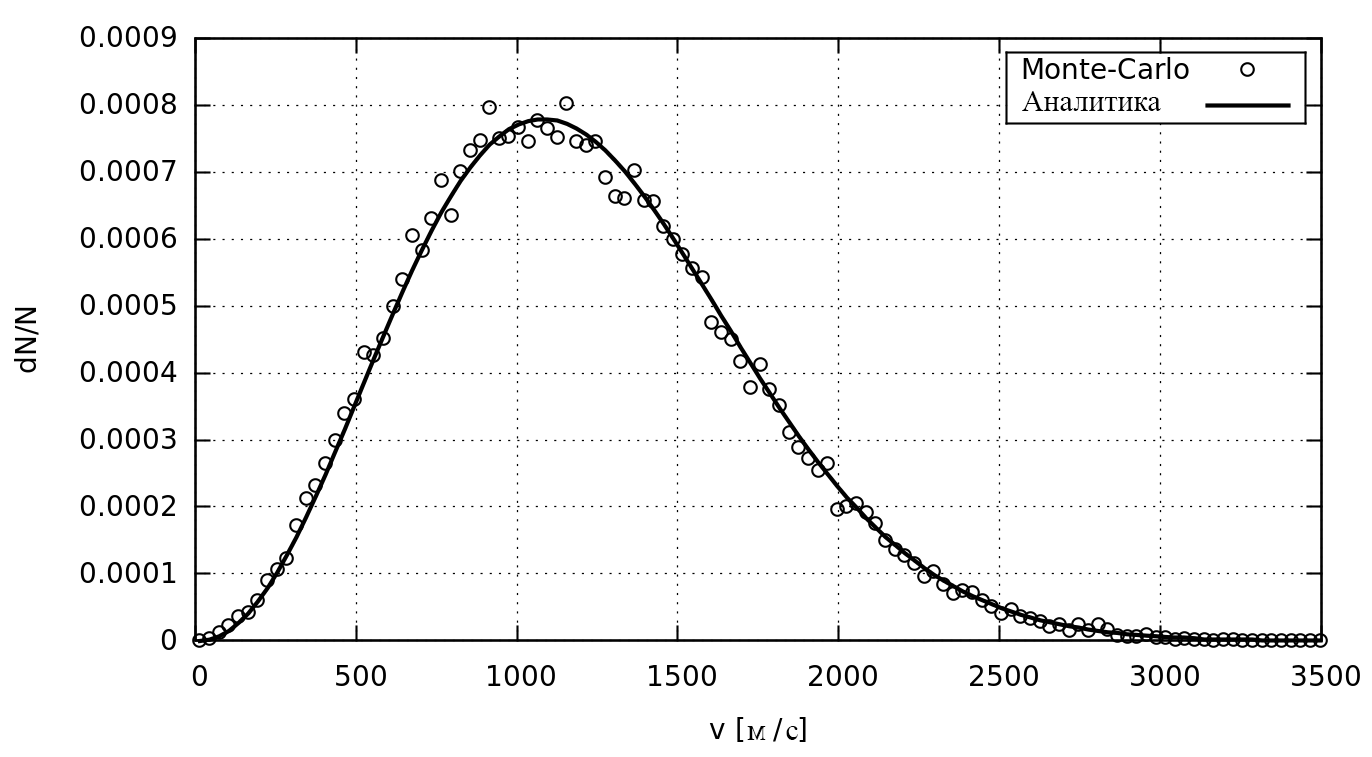
\includegraphics[width=0.85\linewidth]{./fig/ch4/He(T=273)}
\caption{Проверка процедуры задания случайной величины по распределению Максвелла для гелия при $T = 273 \text{ К}$}
\label{fig:He(T=273)}
\end{figure}


